\documentclass{article}
\usepackage{pgfplots}
\usepackage{amsmath}
\usepackage[a4paper,margin=0cm]{geometry}

% Common parameters
\def\samples{1000} % Number of samples for domain resolution
\def\domain{-5:5} % Domain for x values
\def\ymin{-1} % Minimum value for y axis
\def\ymax{6} % Maximum value for y axis
\def\dymin{-0.5} % Minimum value for y axis of derivatives
\def\dymax{1.5} % Maximum value for y axis of derivatives

\begin{document}

\begin{table}[htbp]
    \centering
    \begin{tabular}{p{0.45\linewidth} p{0.45\linewidth}}
        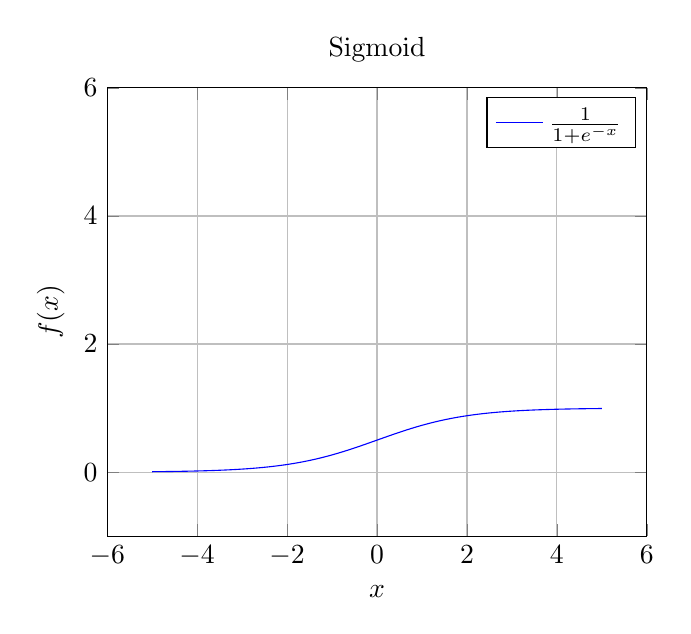
\begin{tikzpicture}
            \begin{axis}[
                xlabel={$x$},
                ylabel={$f(x)$},
                ymin=\ymin, ymax=\ymax,
                grid=both,
                title={Sigmoid},
            ]
            \addplot[blue, domain=\domain, samples=\samples] {1/(1 + exp(-x))};
            \addlegendentry{$\frac{1}{1 + e^{-x}}$}
            \end{axis}
        \end{tikzpicture}
        &
        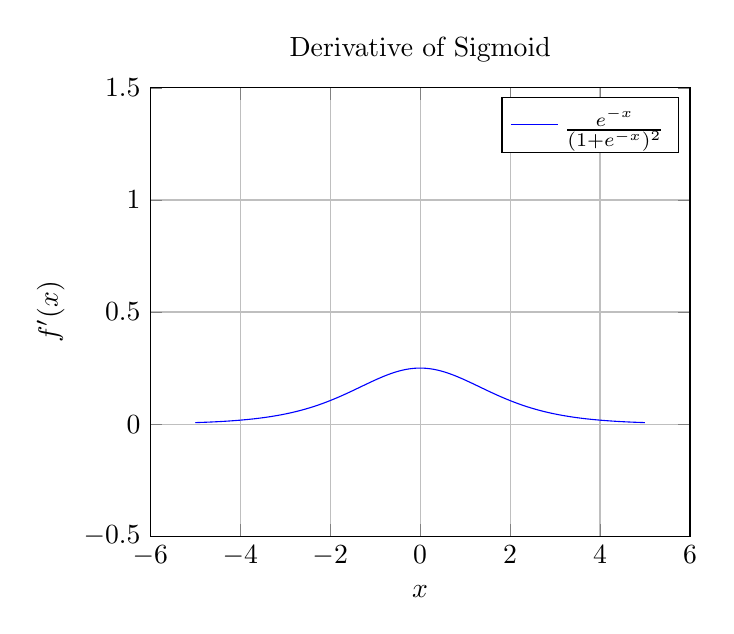
\begin{tikzpicture}
            \begin{axis}[
                xlabel={$x$},
                ylabel={$f'(x)$},
                ymin=\dymin, ymax=\dymax,
                grid=both,
                title={Derivative of Sigmoid},
            ]
            \addplot[blue, domain=\domain, samples=\samples] {1/(1 + exp(-x))*(1-1/(1 + exp(-x)))};
            \addlegendentry{$\frac{e^{-x}}{(1 + e^{-x})^2}$}    
            \end{axis}
        \end{tikzpicture} \\
        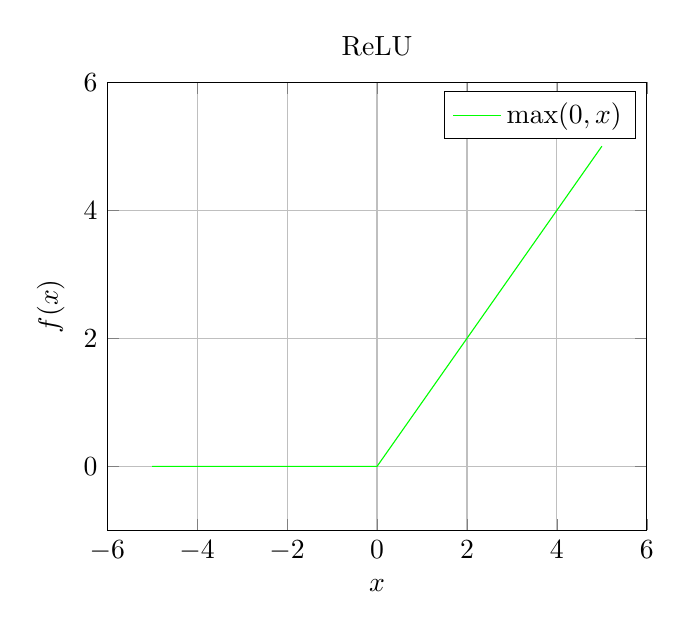
\begin{tikzpicture}
            \begin{axis}[
                xlabel={$x$},
                ylabel={$f(x)$},
                ymin=\ymin, ymax=\ymax,
                grid=both,
                title={ReLU},
            ]
            \addplot[green, domain=\domain, samples=\samples] {max(0,x)};
            \addlegendentry{$\max(0,x)$}
            \end{axis}
        \end{tikzpicture}
        &
        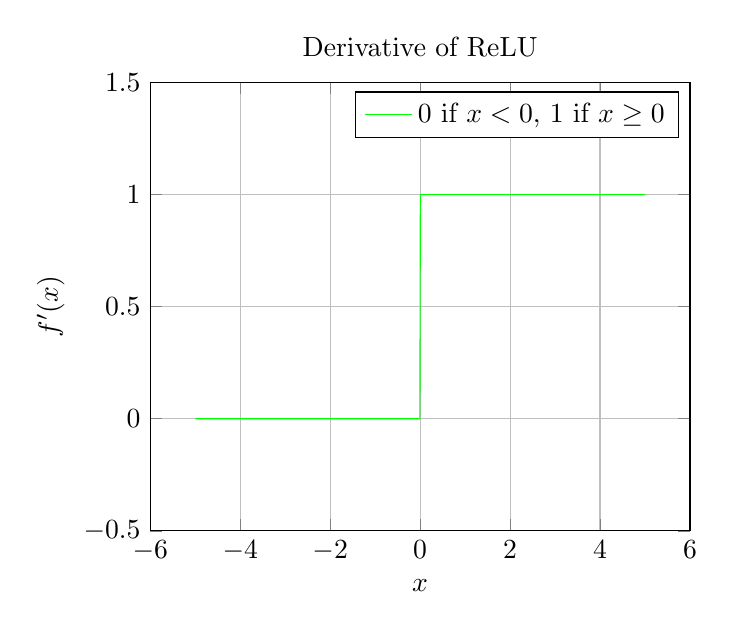
\begin{tikzpicture}
            \begin{axis}[
                xlabel={$x$},
                ylabel={$f'(x)$},
                ymin=\dymin, ymax=\dymax,
                grid=both,
                title={Derivative of ReLU},
            ]
            \addplot[green, domain=\domain, samples=\samples] {x < 0 ? 0 : 1};
            \addlegendentry{$0$ if $x < 0$, $1$ if $x \geq 0$}
            \end{axis}
        \end{tikzpicture}
    \end{tabular}
\end{table}

\end{document}
